\chapter{Механизм поддержания продольных вихрей}

При исследовании модельного порыва определены основные элементы цикла его самоподдержания. Полученные результаты согласуются с существующими представлениями о механизме поддержания организованных структур в пристенных турбулентных течениях. С наличием организованных структур связывают поддержание турбулентных пульсаций \cite{Kim1971}. Основным элементом организованных структур являются полосы повышенной и пониженной скорости, наблюдаемые в пристенной области \cite{Kline1967, Smith1983}. Хотя каждая полоса существует ограниченное время и перемещается вдоль стенки, полосы достаточно хорошо различимы на фоне мелкомасштабных пульсаций. Пульсации могут возникать в результате неустойчивости сдвиговых слоев, существующих в полосчатом течении. Образование полос объясняют наличием продольных вихрей, перемещающих жидкость в нормальной к основному потоку плоскости. Изучению механизма регенерации пристенных структур посвящено большое количество работ \cite{Hamilton1995, Waleffe1995, Waleffe1997, Jimenez1999, Schoppa2002}, но его детали и в первую очередь механизмы образования продольных вихрей в настоящее время не установлены. 

Результаты исследования модельного порыва могут расширить существующие представления о механизме регенерации пристенных структур. В данной главе описан механизм поддержания стационарных продольных вихрей, формирующих полосы в модельном порыве. Также в главе описано решение уравнений Навье-Стокса, имеющее вид бегущей волны, и механизм поддержания продольных вихрей в этом решении. Решение, имеющее вид бегущей волны, периодично вдоль потока и стационарно в сопутствующей системе отсчета. Это решение является предельным состоянием решения, эволюционирующего на сепаратрисе, найденного при тех же условиях симметрии, что и модельный порыв, но в непротяженной расчетной области. Обнаружено, что имея более простое временное поведение, чем модельный порыв, это решение воспроизводит аналогичный механизм самоподдержания. Описание механизма поддержания продольных вихрей на примере решения типа бегущей волны имеет более простой вид и позволяет более строго продемонстрировать особенности движения, обеспечивающие работу этого механизма. 

Основные результаты, представленные в главе, опубликованы в статье автора диссертации \cite{MZG2017, KMU17, KMU16}. 



\section{Получение решения в виде бегущей волны и его свойства}

Пульсационная составляющая движения модельного порыва напоминает бегущую волну. Длину этой волны можно оценить в $5$ радиусов трубы $R$. Соответствующее модельному порыву решение уравнений Навье-Стокса является предельным состоянием решения, эволюционирующего на сепаратрисе, отделяющей области притяжения решений, соответствующих ламинарному и турбулентному режимам течения. Модельный порыв найден при $\Re = 2200$ при дополнительных условиях \eqref{sym_eq}, \eqref{per_eq} в достаточно протяженной расчетной области. Обнаружено, что при дополнительном  условии $5R$-периодичности вдоль трубы решение, эволюционирующее на сепаратрисе, имеет более простое предельное поведение. Предельное решение имеет вид бегущей волны --- оно стационарно в сопутствующей системе отсчета. Решение, имеющее вид бегущей волны, повторяет особенности бегущей волны, наблюдаемой в модельном порыве, и воспроизводит общий с модельным порывом механизм самоподдержания. Фазовая скорость найденной бегущей волны $c_{tw} = 0.77U$ (<<tw>> --- <<traveling wave>>) и близка к фазовой скорости бегущей волны в модельном порыве. Метод поиска решения на сепаратрисе описан в разделе \ref{edge_seq}. 

\begin{figure}
\center{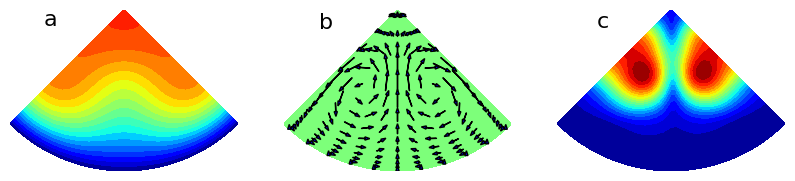
\includegraphics[width=1\linewidth]{pipetw_means.png}}
\center{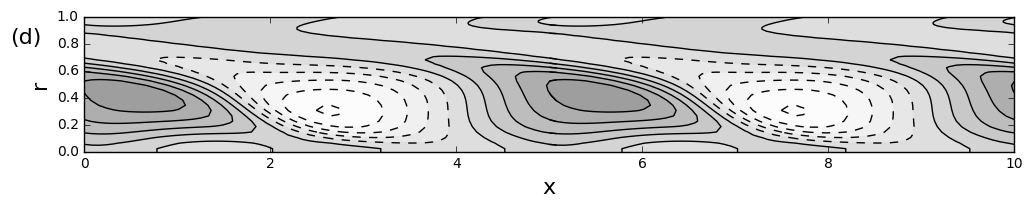
\includegraphics[width=1\linewidth]{pipetw_v1_ls.png}}
\caption{Поле скорости решения, имеющего вид бегущей волны: (a) --- изолинии продольной компоненты $\V_{tw}$ , (b) --- векторное поле поперечной компоненты $\V_{tw}$, (c) --- линии уровня амплитуды пульсаций $\v_{n,tw}$, (d) --- изолинии продольной компоненты $\v_{n,tw}$ в сечении $\theta = 0$. Сплошные линии --- положительные значения, прерывистые --- отрицательные.}
\label{pipetw_pic}
\end{figure}

Как при исследовании модельного порыва, разделим поле скорости бегущей волны $\v_{tw}$ на стационарную $\V_{tw} = \overline{\v_{tw}}^{x}$ и пульсационную $\v_{n,tw} = \v_{tw} - \V_{tw}$ составляющие. В модельном порыве осреднение выполняется по времени в сопутствующей системе отсчета, в которой бегущая волна перемещается вниз по потоку. В случае точной бегущей волны такое осреднение эквивалентно осреднению вдоль трубы. Среднее поле скорости бегущей волны зависят только от $r$ и $\theta$ и является удобным объектом для исследования. 

Продольная и поперечная компоненты среднего поля скорости $\V_{tw}$ изображены на рисунке \ref{pipetw_pic}(a,b). Распределение средней скорости в бегущей волне близко к распределение средней скорости в модельном порыве в области, где пульсации имеют существенную амплитуду (см. рис. \ref{VEL_cs_pic}). На границах расчетной области, где быстрая жидкость проникает ближе к стенке, расположены полосы повышенной скорости; в центре расчетной области, где медленная жидкости находится на большем удалении от стенки --- полоса пониженной скорости. Распределение поперечной скорости соответствует наличию стационарных продольных вихрей, поддерживающих существование полос. Пульсационная составляющая движения бегущей волны $\v_{n,tw}$ также повторяет форму пульсаций, существующих в модельном порыве в области, где эти пульсации имеют существенную амплитуду. На рисунке~\ref{pipetw_pic}(с) представлена амплитуда пульсаций в бегущей волне (амплитуда пульсаций в модельном порыве представлена на рисунке~\ref{puls_cs_pic}). Пульсации сосредоточены между полосами повышенной и пониженной скорости, а также между полосой повышенной скорости и осью трубы. Рисунок \ref{pipetw_pic}(d) позволяет сравнить мгновенное поле скорости пульсационной составляющей движения бегущей волны $\v_{n,tw}$ и модельного порыва~$\v_n$ (см. рис. \ref{lin_ls_cmp_pic}). На рисунках изображена продольная компонента скорости в одном из продольных сечений трубы $\theta = 0$, в котором пульсации имеют существенную амплитуду. 

\begin{figure}
\center{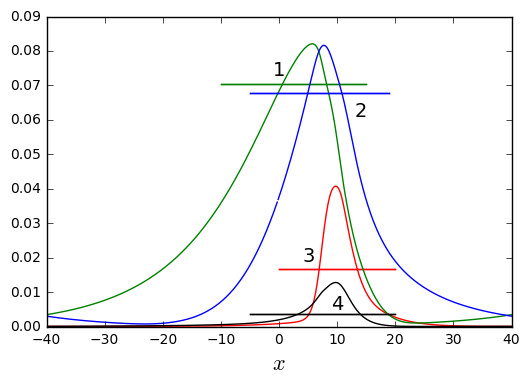
\includegraphics[width=0.5\linewidth]{pipetw_amp.png}}
\caption{Средние по сечению трубы амплитуды компонент движения бегущей волны (не зависят от $x$) и модельного порыва (функции $x$): 1 --- $\V_S$; 2 --- $\V_{2D}$ (отклонение от течения Пуазейля); 3 --- $\v_n$; 4 --- $\V_V$.}
\label{pipetw_amp_pic}
\end{figure}

Найденная бегущая волна повторяет качественные особенности модельного порыва, но количественно наблюдаются существенные отличия. Для сравнения на рисунке \ref{pipetw_amp_pic} приведены средние по сечению трубы амплитуды компонент движения бегущей волны и модельного порыва. Для бегущей волны приведенные величины не зависят от продольной координаты. Графики для модельного порыва повторяют графики, приведенные на рисунке~\ref{amp_pic}. По аналогии с модельным порывом, среднее течение $\V_{tw}$ представлено в виде суммы двумерной $\V_{2D,tw} = \overline{\V_{tw}}^\theta$ и трехмерной  $\V_{3D,tw} = \V_{tw} - \V_{2D,tw}$ составляющих. Трехмерная составляющая движения разложена на продольную $\V_{S,tw}$ и поперечную $\V_{V,tw}$ компоненты, ассоциированные с полосами и продольными вихрями. Соотношения между интенсивностью различных компонент движения в бегущей волне сохраняется, но абсолютные значения оказываются значительно ниже. Наибольшее отличие наблюдается в интенсивности среднего поперечного движения $\V_V$. В бегущей волне значение амплитуды этого движения почти в четыре раза ниже наибольшего значения, достигаемого в модельном порыве. Это можно объяснить исходя из представлений о том, что решение на сепаратрисе является равновесным, и интенсивность продольны вихрей определяется необходимость поддержания полос. В бегущей волне продольные вихри и полосы существует во всем течении. В модельном порыве протяженность продольных вихрей оказывается значительно ниже протяженности полос, соответственно для поддержания полос вихри в этом случае должны иметь большую интенсивность. 


\begin{figure}
\center{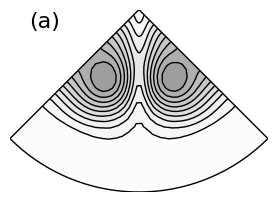
\includegraphics[width=0.33\linewidth]{pipetw_lin_amp.png} 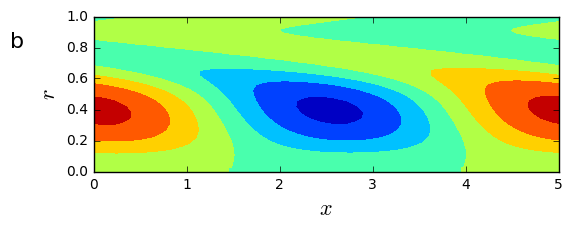
\includegraphics[width=0.6\linewidth]{pipetw_lin_ls.png}}
\caption{Наиболее быстро растущее собственное решение линейной задачи устойчивости поля скорости $\V_{tw}$: (a) --- линии уровня амплитуды колебаний; (b) --- изолинии продольной компоненты скорости в сечении $\theta = 0$. Сплошные линии --- положительные значения, прерывистые --- отрицательные.}
\label{pipetw_lin_pic}
\end{figure}


Также, как в модельном порыве, пульсационная составляющая движения бегущей волны $\v_{n,tw}$ возникает в результате линейной неустойчивости среднего течения $\V_{tw}$. Наиболее быстро растущее собственное решение линейной задачи устойчивости поля скорости $\V_{tw}$ повторяет форму пульсационной составляющей движения и её фазовую скорость. Соответствующий инкремент нарастания $\lambda = 0.0085R/U$. Для сравнения с пульсационной составляющей движения $\v_{n,tw}$, поле скорости которой представлено на рисунке \ref{pipetw_pic}(c,d), на рисунке \ref{pipetw_lin_pic}(a,b) приведены амплитуда колебаний наиболее быстро растущего решения линейной задачи устойчивости и его мгновенное поле скорости в продольном сечении трубы. Также, как для модельного порыва, для бегущей волны полученные в рамках линеаризованных уравнений пульсации имеют дополнительную симметрию отражения относительно сечения $\theta = \pi/4$, выражаемую уравнением \eqref{dop_sym_eq}. Пульсации достигают своего максимума между полосами повышенной и пониженной скорости. В этой области находится точка перегиба, если рассматривать среднее течение как функцию переменной~$\theta$. Вероятным механизмом образования пульсаций является механизм типа Кельвина-Гельмгольца.

%\lambda = - 0.0065

Получено решение уравнений Навье-Стокса в виде бегущей волны, описаны его основные свойства. Это решение воспроизводит основные элементы цикла поддержания модельного порыва, но имеет более простую форму. Поле скорости бегущей волны стационарно в сопутствующей системе отсчета. Осреднение вдоль трубы позволяет разделить его на среднюю и пульсационную составляющие. Показано, что пульсационная составляющая движения возникает в результате линейной неустойчивости среднего течения. Неустойчивость связана с наличием в среднем течении полос повышенной и пониженной скорости. Существование полос поддерживают стационарные продольные вихри. В следующих двух главах представлен механизм поддержания продольных вихрей, замыкающий цикл поддержания колебаний в этом решении. 


\section{Механизм поддержания продольных вихрей на примере решения в виде бегущей волны}

Принято считать, что продольные вихри, ответственные за образование полос в пристенных турбулентных течениях, возникают в результате некоторого нелинейного взаимодействия пульсаций, однако детали такого взаимодействия не установлены. Прояснить процесс формирования продольных вихрей в рассматриваемых модельных течениях позволяет анализ уравнения, описывающего эволюцию продольной завихренности, полученного применением оператора ротора к уравнению Навье-Стокса \eqref{NS_eq}:
\begin{equation}\label{ox_eq}
\pd{\omega_x}{t} - \nu\Laplace \omega_x =  c_{f} \pd{\omega_x}{x} -  (\v \nabla) \omega_x + (\om \nabla) v_x.
\end{equation}
Здесь $\om = (\omega_x, \omega_r, \omega_\theta) = \rot \v$ --- вектор завихренности, $c_{f}$ --- скорость перемещения системы отсчета. Уравнение для стационарной составляющей продольной завихренности получается после осреднения \eqref{ox_eq} вдоль трубы:
\begin{equation}\label{OX_eq}
\pd{\Omega_x}{t} + (\V \nabla) \Omega_x - \nu\Laplace \Omega_x = - \overline{(\v' \nabla) \omega'_x}^x + \overline{ (\om' \nabla) v'_x }^x.
\end{equation}
Здесь  $\Om=(\Omega_x, \Omega_r, \Omega_\theta) = \overline{\om}^x$ и $\om'=(\omega'_x, \omega'_r, \omega'_\theta) = \om - \Om$ --- средняя и пульсационная составляющие вектора завихренности. Слагаемые в правой части уравнения \eqref{OX_eq} отвечают за генерацию $\Omega_x$, обусловленную нелинейным взаимодействием пульсаций. Слагаемые в левой части уравнения отвечают за конвекцию существующей $\Omega_x$ и вязкие эффекты. Так как среднее течение во времени не меняется, источниковые слагаемые в правой части уравнения \eqref{OX_eq} компенсируются конвективным и вязким слагаемыми в левой его части. 

В скалярных переменных уравнение \eqref{OX_eq} имеет вид:
\begin{multline}\label{OX1_eq}
\pd{\Omega_x}{t} + V_r \pd{\Omega_x}{r} + \frac{V_\theta}{r} \pd{\Omega_x}{\theta}
 - \nu\left(\pd{^2\Omega_x}{r^2} + \frac{1}{r^2}\pd{^2\Omega_x}{\theta^2} + \frac{1}{r}\pd{\Omega_x}{r}\right)= \\
 - \overline{v'_x \pd{\omega'_x}{x}}^x - \overline{v'_r \pd{\omega'_x}{r}}^x - \overline{\frac{v'_\theta}{r} \pd{\omega'_x}{\theta}}^x
 + \overline{\omega'_x \pd{v'_x}{x}}^x + \overline{\omega'_r \pd{v'_x}{r}}^x + \overline{\frac{\omega'_\theta}{r} \pd{v'_x}{\theta}}^x.
\end{multline}
Для выявления определяющих механизмов генерации средней продольной завихренности удобнее рассмотреть уравнение эволюции квадрата $\Omega_x$, получающееся домножением всех членов \eqref{OX1_eq} на $2\Omega_x$. Положительный или отрицательный знак у полученных таким образом выражений в правой части уравнения показывает соответственно положительный или отрицательный вклад этого члена в изменение $\Omega_x^2$, а, следовательно, и в интенсивность поперечного движения. Распределение $\Omega_x^2$ по сечению трубы представлено на рисунке~\ref{OXgen_pic}(a). В большей части трубы средняя продольная завихренность близка к нулю. Области концентрации $\Omega_x$ находятся между полосами повышенной и пониженной скорости и соответствуют наличию стационарных продольных вихрей (см. рис. \ref{pipetw_pic}(b)). 

Анализ уравнения \eqref{OX1_eq} показал, что два слагаемых в правой части этого уравнения вносят определяющий вклад в производство средней продольной завихренности. Эти слагаемые имеют вид:
\begin{equation}\label{OXgen_terms}
- \overline{v'_x \frac{\d \omega'_x}{\d x}}^x + \overline{ \omega'_x \frac{\d v'_x}{\d x} }^x.
\end{equation}
Слагаемые \eqref{OXgen_terms} описывают нелинейное взаимодействие пульсаций продольной скорости $v'_x$ и пульсаций продольной завихренности $\omega'_x$. Между собой выделенные слагаемые равны в силу периодичности решения вдоль трубы. Слагаемые \eqref{OXgen_terms}, умноженные на $2\Omega_x$, представлены на рисунке~\ref{OXgen_pic}(b), на рисунке~\ref{OXgen_pic}(c) приведена сумма других слагаемых в правой части \eqref{OX_eq}, также умноженная на $2\Omega_x$. Вклад слагаемых \eqref{OXgen_terms} определяет форму поля $\Omega_x^2$ и более чем на порядок превосходит суммарный вклад других источниковых членов. Таким образом, нет сомнения в том, что стационарные продольные вихри возникают за счет действия выделенной пары слагаемых.

\begin{figure}
\center{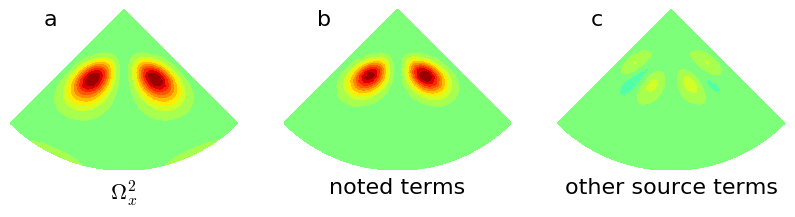
\includegraphics[width=1\linewidth]{pipetw_OXgen.png}}
\caption{Распределение по сечению трубы $\Omega_x^2$ (a) и вклад в генерацию $\Omega_x^2$ со стороны слагаемых, соответствующих слагаемым \eqref{OXgen_terms} (b) и другим слагаемым в правой части \eqref{OX_eq} (с). Сплошные линии соответствуют положительным значениям, прерывистые --- отрицательным.}
\label{OXgen_pic}
\end{figure}

Отметим, что пульсации, соответствующие старшей собственной функции линейной задачи об устойчивости среднего стационарного течения, также демонстрируют приведенный выше механизм образования стационарных продольных вихрей. Важно, что это наблюдается только в том случае, когда при анализе устойчивости учитываются как продольная, так и поперечная составляющие среднего течения. Принято считать, что поперечное движение, определяя угловую неоднородность в распределении продольной скорости среднего течения, не может существенным образом влиять на свойства его устойчивости вследствие незначительности своей амплитуды. Поэтому при исследовании линейной устойчивости подобных течений, например, полосчатых структур в турбулентных потоках, наличие поперечного движения обычно не принимается во внимание. В нашем случае пренебрежение поперечным движением приводит к тому, что стационарное течение оказывается линейно устойчивым. Что еще более важно, наименее затухающее возмущение не воспроизводит при этом описанный механизм формирования продольных вихрей. Это связанно с тем, что форма пульсаций продольной завихренности $\omega'_x$ качественно меняется, хотя пульсации продольной скорости $v'_x$ сохраняют свою форму практически неизменной. Тем самым нарушается согласованность  $v'_x$ и $\omega'_x$, необходимая для обеспечения нужного вклада выражения \eqref{OXgen_terms} в производство продольной завихренности.

\begin{figure}
\center{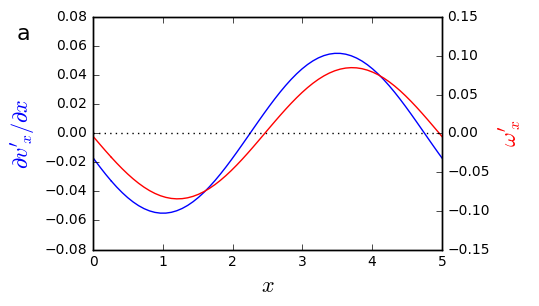
\includegraphics[width=0.5\linewidth]{pipetw_lin_cor.png}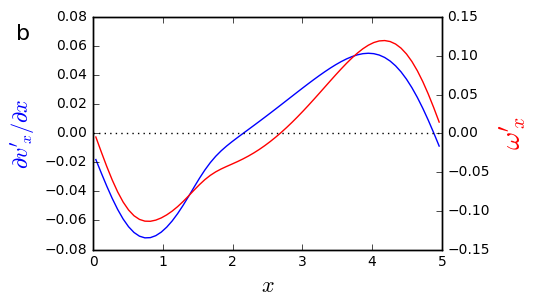
\includegraphics[width=0.5\linewidth]{pipetw_puls_cor.png}}
\caption{Значение $\d v_x' /\d x$ (кривая 1) и $\omega_x'$ (кривая 2) на прямой, проходящей через область, занятую положительным вихрем, при $r = 0.5, \theta = \pi/8$: (a) --- для пульсаций, полученных в линейном приближении; (b) --- для пульсационной составляющей движения бегущей волны. }
\label{OXgen_corr_pic}
\end{figure}

Интересно отметить, что сумма слагаемых \eqref{OXgen_terms}, посчитанных для собственного решения линейной задачи устойчивости поля скорости $\V_{tw}$, не зависит от $x$. В линейном приближении слагаемые \eqref{OXgen_terms}, поддерживая существование продольных вихрей, сохраняют их независящими от продольной координаты. Среднее поле скорости $\V_{tw}$ однородно вдоль трубы, следовательно, возникающие на нем собственные возмущения меняются вдоль трубы по гармоническом закону. При фиксированных значениях $r$ и $\theta$ пусть  $v'_x = a \sin(\alpha x + \phi)$, $\omega_x' = b \sin(\alpha x + \psi)$, тогда:
\begin{equation*} \label{OXgen_iterms_1}
 - v'_x \frac{\d \omega'_x}{\d x} = - \alpha a b \sin(\alpha x + \phi) \cos(\alpha x + \psi),
\end{equation*}
\begin{equation*} \label{OXgen_iterms_2}
\omega'_x \frac{\d v'_x}{\d x} =  \alpha a b \cos(\alpha x + \phi) \sin(\alpha x + \psi),
\end{equation*}
\begin{equation} \label{OXgen_iterms_sum}
 - v'_x \frac{\d \omega'_x}{\d x} + \omega'_x \frac{\d v'_x}{\d x} = \alpha a b \sin(\psi - \phi).
\end{equation}
Сумма \eqref{OXgen_iterms_sum} не зависит от $x$, что, в частности, позволяет упустить знак осреднения вдоль трубы. Эффективность производства  $\Omega_x$ определяется разностью фаз $\psi - \phi$. В области положительного вихря, при $a,b > 0$, наибольшее значение как первого, так и второго слагаемого достигается при $\psi - \phi = \pi/2$. В этом случае $\d \omega'_x/\d x$ и $v'_x$ положительно коррелированы, в то время как $\d v'_x/\d x$ и $\omega'_x$ --- отрицательно. В области отрицательного вихря ситуация меняется на противоположную. Расчет соответствующих коэффициентов корреляции показывает, что они близки к $\pm1$ в соответствующих областях. В качестве подтверждения на рисунке \ref{OXgen_corr_pic}(a) представлены значения $\d v'_x/\d x$ и $\omega'_x$ на прямой, проходящей через область, занятую положительным вихрем, $r = 0.5, \theta = \pi/8$. Фазы выделенных компонент движения практически совпадают. Указанное свойство сохраняется также для пульсационной составляющей движения $\v'_{tw}$, для которой аналогичные величины изображены на рисунке \ref{OXgen_corr_pic}(b). Объяснить наблюдаемую согласованность фаз позволяет механизм образования пульсаций продольной завихренности, представленный в следующем разделе. 


\section{Механизм поддержания пульсаций продольной завихренности на примере решения в виде бегущей волны}

Объяснить согласованность фаз между пульсациями продольной скорости и завихренности, необходимой для работы механизма образования продольных вихрей, позволяет анализ уравнения эволюции $\omega'_x$, полученного вычитанием \eqref{OX_eq} из \eqref{ox_eq}:
\begin{multline}\label{ox1_eq}
\pd{\omega'_x}{t} - c_f\pd{\omega'_x}{x} + (\V\nabla) \omega'_x - \nu \nabla^2 \omega'_x = - (\v'\nabla) \Omega_x
+(\Om\nabla) v'_x + (\om'\nabla) V_x - \\ - (\v'\nabla) \omega'_x  + (\om'\nabla) v'_x  + \overline{(\v'\nabla) \omega'_x}^x  - \overline{(\om'\nabla)v'_x}^x.
\end{multline}
В скалярных переменных уравнение \eqref{ox1_eq} имеет вид:
\begin{multline}\label{ox2_eq}
\pd{\omega'_x}{t} + (V_x - c_f)\pd{\omega'_x}{x} + V_r \pd{\omega_x'}{r} + \frac{V_\theta}{r} \pd{\omega'_x}{\theta} 
- \nu\left(\pd{^2\omega'_x}{x^2} + \pd{^2\omega'_x}{r^2} + \frac{1}{r^2}\pd{^2\omega'_x}{\theta^2} + \frac{1}{r}\pd{\omega'_x}{r}\right) = \\
- v'_r \pd{\Omega_x}{r} - \frac{v'_\theta}{r} \pd{\Omega_x}{\theta} 
+ \Omega_x \pd{v'_x}{x} + \Omega_r \pd{v'_x}{r} + \frac{\Omega_\theta}{r} \pd{v'_x}{\theta}
+ \omega'_r \pd{V_x}{r} + \frac{\omega'_\theta}{r} \pd{V_x}{\theta} - \\ 
- v'_x \pd{\omega'_x}{x} - v'_r \pd{\omega'_x}{r} - \frac{v'_\theta}{r} \pd{\omega'_x}{\theta} 
+ \omega'_x \pd{v'_x}{x} + \omega'_r \pd{v'_x}{r} + \frac{\omega'_\theta}{r} \pd{v'_x}{\theta} + \\
+ \overline{v'_x \pd{\omega'_x}{x}}^x + \overline{v'_r \pd{\omega'_x}{r}}^x + \overline{\frac{v'_\theta}{r} \pd{\omega'_x}{\theta}}^x
- \overline{\omega'_x \pd{v'_x}{x}}^x - \overline{\omega'_r \pd{v'_x}{r}}^x - \overline{\frac{\omega'_\theta}{r} \pd{v'_x}{\theta}}^x.
\end{multline}
Удобнее работать с уравнением, описывающим изменение среднего квадрата пульсаций продольной завихренности $\overline{\omega'_x\omega'_x}^x$, получающимся умножением каждого из слагаемых в \eqref{ox2_eq} на~$2\omega'_x$ c последующим осреднением вдоль трубы. Слагаемые в этом уравнении не зависят от времени и продольной координаты. Сумма слагаемых в правой части уравнения компенсируется вязкими и конвективными членами в левой части. Как и в предыдущем случае, в правой части уравнения удается выделить существенные слагаемые, ответственные за возникновение пульсаций~$\omega'_x$. 


Распределение $\overline{\omega'_x \omega'_x}^x$ по сечению трубы изображено на рисунке~\ref{ox1gen_pic}(a). Основные пульсации $\omega'_x$ наблюдаются в центре расчетной области около оси трубы. На месте расположения продольных вихрей также присутствуют пульсации $\omega'_x$, но меньшей интенсивности. В остальной части трубы их амплитуда близка к нулю. Обнаружено, что за генерацию пульсаций $\omega'_x$ в центральной части трубы и на месте продольных вихрей отвечают два разных механизма. Первый дает пульсации большей амплитуды, однако, за возникновение стационарных продольных вихрей ответственны пульсации, производимые вторым механизмом, так как именно они оказываются согласованными с пульсациями $v'_x$ нужным образом.


\begin{figure}
\center{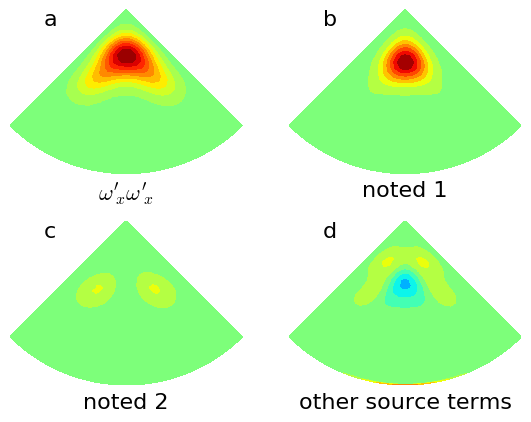
\includegraphics[width=0.66\linewidth]{pipetw_ox1gen.png}}
\caption{Распределение по сечению трубы среднего квадрата пульсаций продольной завихренности $\overline{\omega'_x \omega'_x }^x$ (а) и вклад в его производство со стороны слагаемых \eqref{ox1gen_add_terms} (b), слагаемого \eqref{ox1gen_main_terms} (c) и суммы остальных слагаемых в правой части \eqref{ox1_eq} (d). Сплошные линии --- положительные значения, прерывистые --- отрицательные.}
\label{ox1gen_pic}
\end{figure}


Первый механизм формирования~$\omega'_x$ связан с наличием нормальных к стенке вихрей в пульсационной составляющей движения. Цепочка нормальных к стенке вихрей, чередующихся по знаку, двигается вниз по полосе пониженной скорости. Этим вихрям соответствуют области повышенной амплитуды пульсаций радиальной завихренности~$\omega'_r$. На рисунке \ref{pipetw_or1_pic} приведено значение~$\omega'_r$ в сечении $r = 0.5$, нормальном к выделенной компоненте завихренности. Приведенные на \ref{pipetw_or1_pic}(a) значения посчитаны по пульсациям, полученным в рамках линеаризованных уравнений. Аналогичные значения для пульсационной составляющей движения $\v_{n,tw}$ представлены на рисунке \ref{pipetw_or1_pic}(b). Амплитуда~$\omega'_x$ оказывается на порядок ниже амплитуды~$\omega'_r$, амплитуда~$\omega'_\theta$ в центральной части трубы равна нулю в силу симметрии. Таким образом, в центральной части трубы поле завихренности представлено в первую очередь радиальной компонентой и соответствует нормальным к стенке вихрям.

Пульсации продольной завихренности $\omega'_x$ возникают вследствие поворота нормальных к стенке вихрей, происходящего в присутствии градиента продольной скорости $\d V_x/ \d r$, возникающего между полосой замедления и осью трубы. Кроме того, наличие радиального градиента $\d V_x/ \d r$ связано с наличием угловой завихренности $\Omega_\theta = \d V_r / \d x - \d V_x / \d r$. Радиальная пульсационная завихренность $\omega'_r = \d v'_x / r \d \theta - \d v'_\theta / \d x$ за счет первого из слагаемых поворачивает стационарные угловые вихри так, что те также приобретают пульсационную продольную составляющую. В уравнении \eqref{ox1_eq} за описанный механизм отвечают слагаемые:
\begin{equation}\label{ox1gen_add_terms}
\frac{\d \omega'_x}{\d t} = \omega'_r \frac {\d V_x}{\d r} + \frac{\Omega_\theta}{r} \frac{\d v'_x}{\d \theta} + ...
\end{equation}
Несмотря на то, что выделенные в \eqref{ox1gen_add_terms} слагаемые имеют противоположные знаки и в значительной степени компенсируют друг друга при сложении, их вклад в производство $\omega'_x$ значителен (смотри рисунок~\ref{ox1gen_pic}(b)). Они определяют форму пульсаций $\omega'_x$ в области между полосой замедления и осью трубы, где пульсации $\omega'_x$ достигают наибольшего значения. Эти пульсации, однако, практически не участвуют в образовании стационарной составляющей продольной завихренности. Это объясняется тем, что колебания $\omega'_x$, рождающиеся в результате описанного механизма, близки по фазе к колебаниям $v'_x$, так что каждое из слагаемых в выражении \eqref{OXgen_terms} при осреднении дает близкое к нулю значение.

\begin{figure}
\center{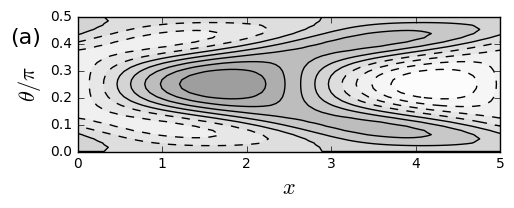
\includegraphics[width=0.45\linewidth]{pipetw_or1_lin.png} 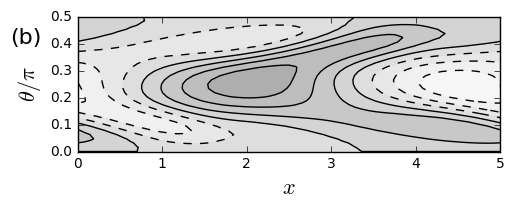
\includegraphics[width=0.45\linewidth]{pipetw_or1.png}}
\caption{Линии уровня нормальной к стенке компоненты завихренности $\omega_r'$ в сечении $r = 0.5$ для пульсаций, полученных в рамках линейного приближения (а) и для пульсационной составляющей движения бегущей волны (b). Сплошные линии --- положительные значения, прерывистые --- отрицательные.}
\label{pipetw_or1_pic}
\end{figure}

Второй механизм образования пульсаций продольной завихренности $\omega'_x$ связан с перераспределением уже существующей стационарной продольной завихренности $\Omega_x$ за счет пульсационной составляющей продольной скорости $v'_x$ (эффект сжатия/растяжения вихревых линий). В уравнении \eqref{ox1_eq} за описываемый механизм отвечает слагаемое
\begin{equation}\label{ox1gen_main_terms}
\frac{\d \omega'_x}{\d t} = \Omega_x \frac {\d v'_x}{\d x} + ...
\end{equation}
Выделенное в \eqref{ox1gen_main_terms} слагаемое стремится произвести пульсации $\omega'_x$, пропорциональные $\d v'_x / \d x$, причем коэффициентом пропорциональности выступает средняя продольная завихренность. Соответственно,  механизм включается в областях концентрации~$\Omega_x$. В области расположения положительного вихря производимые пульсации $\omega'_x$ положительно пропорциональны пульсациям $\d v'_x / \d x$, а в области расположения отрицательного вихря --- отрицательно пропорциональны. Таким образом обеспечивается максимально возможная эффективность производства средней продольной завихренности нужного знака посредством второго из слагаемых \eqref{OXgen_terms}. Пульсации $-v'_x$ и $\d \omega'_x / \d x$ отказываются также согласованы нужным образом, так что первое слагаемое \eqref{OXgen_terms} равно второму.

На рисунке~\ref{ox1gen_pic}(c) приведен вклад выделенного в \eqref{ox1gen_main_terms} слагаемого в производство $\overline{\omega'_x \omega'_x}^x$. Это слагаемое определяет форму пульсаций в области существования продольных вихрей --- между полосами повышенной и пониженной скорости. Суммарный вклад других слагаемых в правой части \eqref{ox1_eq}, не попавших на рисунки~\ref{ox1gen_pic}(b,c), изображен на рисунке~\ref{ox1gen_pic}(d). Эти слагаемые также поддерживают существование колебаний в области расположения продольных вихрей, но их влияние оказывается значительно ниже влияния выделенного в \eqref{ox1gen_main_terms} слагаемого. В точке, где $\Omega_x$ достигает максимума, приведенная на рисунке (d) величина оказывается в три раза ниже приведенной на рисунке (c). Стоит также учитывать, что пульсации, генерируемые слагаемыми, которым соответствует рисунок (d), не обязательно согласованы по фазе с пульсациями продольной скорости нужным для поддержания продольных вихрей образом, так что роль слагаемых (d) в поддержании продольных вихрей может оказаться еще ниже. 

Пульсации продольной завихренности, согласованные с пульсациями продольной скорости необходимым для поддержания продольных вихрей образом, имеют наибольшую амплитуду в области образования пульсационной составляющей движения, между полосами повышенной и пониженной скорости, по нескольким причинам. Во-первых, в этой области пульсации продольной скорости, ответственные за образование пульсаций продольной завихренности, также имеют наибольшую амплитуду. Во вторых, в этой области средняя скорость течения близка к фазовой скорости пульсаций, благодаря чему сформированные пульсации $\omega'_x$, сносимые вниз по потоку основным течением, сохраняют согласованность фаз с производящими их пульсациями $\partial v_x'/\partial x$. Потеря согласованности фаз привела бы к невозможности дальнейшего роста $\omega'_x$. Продольные вихри располагаются в области возникновения пульсаций, между полосами повышенной и пониженной скорости, так как именно в этой области пульсации продольной скорости и пульсации продольной завихренности имеют наибольшую амплитуду. Таким образом продольные вихри оказываются расположены наиболее удачным образом для поддержания существования этих полос. 

Описанный механизм генерации пульсаций продольной завихренности объясняет необходимость учета поперечного движения при исследовании устойчивости стационарного течения. Пренебрежение связанной с поперечным движением $\Omega_x$ делает невозможным генерацию $\omega'_x$ в форме, необходимой для сохранения поперечного движения, а следовательно и всего процесса самоподдержания пульсаций.


\section{Механизм поддержания продольных вихрей и пульсаций продольной завихренности в модельном порыве}

Выделенный при изучении бегущей волны, возникающей в непротяженной расчетной области, механизм образования продольных вихрей может быть обобщен на модельный порыв. В этом случае разделение движения на среднюю и пульсационную составляющие выполняется путем осреднения по времени в системе отсчета, связанной с порывом. Для точной бегущей волны такое осреднение эквивалентно осреднению вдоль трубы. Осреднение по времени позволяет получить те же результаты для точной бегущей волны, и близкие результаты для бегущей волны, выделяемой в модельном порыве. 

Разделим поле скорости модельного порыва $\v_{mp}$ на среднюю $\V_{mp} = \overline{\v_{mp}}^t$ и пульсационную $\v'_{mp} = \v_{mp} - \V_{mp}$ составляющие (<<mp>> --- <<model puff>>). Соответственно, завихренность стационарной и пульсационной составляющих движения обозначим $\Om_{mp} = \rot \V_{mp}$ и $\om'_{mp} = \rot \v'_{mp}$. Отметим, что завихренность стационарной составляющей движения равна стационарной составляющей поля завихренности: $\Om = \overline{\om}^t$, где $\om = \rot \v$ --- поле завихренности. Аналогично, завихренность пульсационной составляющей движения равна пульсационной составляющей поля завихренности: $\om' = \om - \Om$. 

Как и в случае бегущей волны, стационарная составляющая поля скорости модельного порыва воспроизводит продольные вихри (смотри рисунок \ref{VEL_cs_pic}). В расчетную область попадает пара таких вихрей. Они ответственны за образование полос повышенной и пониженной скорости. Для того, чтобы установить механизм образования продольных вихрей, обратимся к уравнению, описывающему изменение продольной завихренности \eqref{ox_eq}. Его осреднение по времени позволяет получить уравнение баланса стационарной составляющей продольной завихренности $\Omega_x$, имеющее в данном случае вид:
\begin{equation} \label{time_OX_eq}
\pd{\Omega_x}{t} - \nu\nabla^2 \Omega_x = - (\V - \c_f, \nabla) \Omega_x + (\Om, \nabla) V_x - \overline{(\v', \nabla) \omega'_x}^t + \overline{ (\om', \nabla) v'_x }^t.
\end{equation}
Уравнение \eqref{time_OX_eq} аналогично уравнению \eqref{OX_eq} за тем исключением, что в этом случае осреднение производится по времени. Слагаемые в правой части \eqref{time_OX_eq} можно рассматривать как источники $\Omega_x$. Они <<наполняют>> функцию $\Omega_x$ до тех пор, пока их действие не уравновесит вязкость. Среди них могут быть выделены слагаемые, определяющие форму поля $\Omega_x$, связанные с механизмом его формирования. Удобнее работать с уравнением баланса квадрата стационарной продольной завихренности $\Omega_x^2$, полученным скалярным умножением \eqref{time_OX_eq} на $2\Omega_x$. Положительное или отрицательное значение источниковых членов в этом уравнении говорит о положительном или отрицательном их влиянии на образование $\Omega_x$. 


\begin{figure}[h]
\center{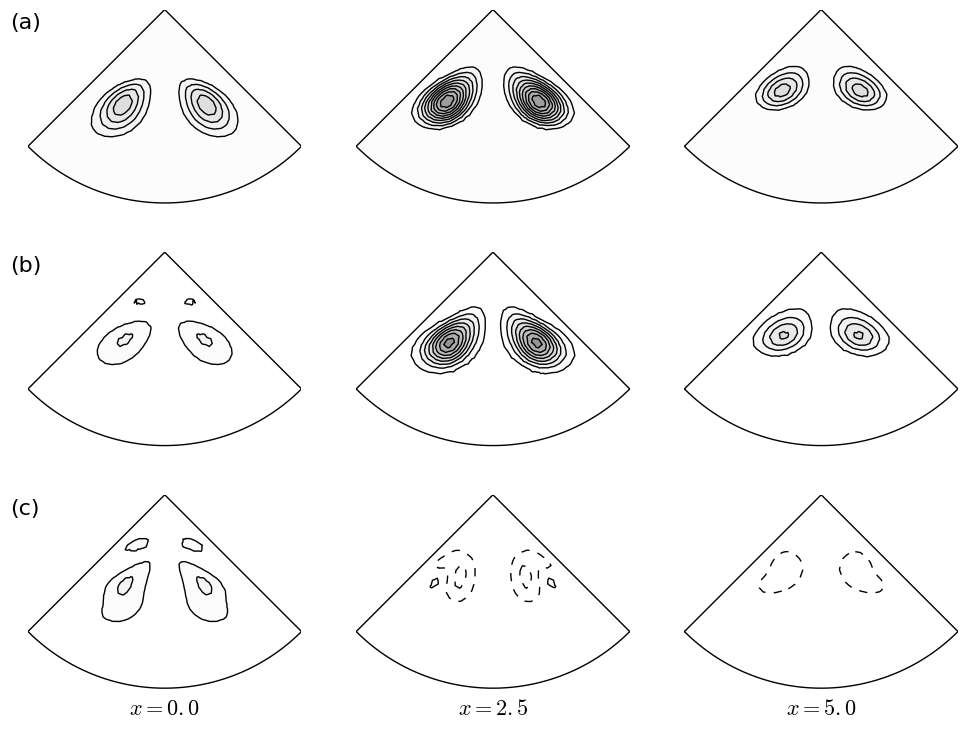
\includegraphics[width=1\linewidth]{puff_OXgen.png}}
\caption{В нескольких сечения трубы приведено значение $\Omega_x^2$ (ряд (а)), а также вклад в образование $\Omega_x^2$ со стороны \eqref{time_OXgen_terms} (ряд (b)) и других слагаемых в правой части уравнения \eqref{time_OX_eq} (ряд (c)). Представлено три сечения из области существования продольных вихрей, $x=0,2.5,5$. Сплошные изолинии соответствуют положительным значениям, прерывистые --- отрицательным.}
\label{mp_OXgen_pic}
\end{figure}

Анализ уравнения \eqref{time_OX_eq} позволил установить механизм образования стационарных продольных вихрей аналогичный выделенному при изучении бегущей волны. За образование продольных вихрей в этом случае ответственна пара слагаемых, сохраненная в уравнении ниже: 
\begin{equation} \label{time_OXgen_terms}
\pd{\Omega_x}{t} = - \overline{v'_x \pd{\omega'_x}{x}}^t + \overline{\omega'_x \pd{v'_x}{x}}^t + ... 
\end{equation}
Слагаемые \eqref{time_OXgen_terms} соответствуют слагаемым \eqref{OXgen_terms}, выделенным при изучении бегущей волны. На рисунке \ref{mp_OXgen_pic} в ряду (а) представлен квадрат продольной завихренности $\Omega_x^2$ в трех сечениях трубы. Его распределение соответствует паре продольных вихрей, расположенных по бокам от полосы замедления (проходящей через центр расчетной области). На рисунке \ref{mp_OXgen_pic} в рядах (b) и (с) в тех же сечения приведен вклад \eqref{time_OXgen_terms} и других слагаемых в правой части уравнения \eqref{time_OX_eq} в образование $\Omega_x^2$. Вклад слагаемых \eqref{time_OXgen_terms} значительно превосходит по величине вклад других слагаемых почти во всех сечениях, он повторяет и определяет форму поля $\Omega_x$. 

\begin{figure}
\center{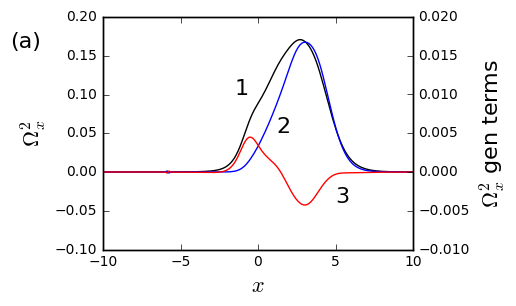
\includegraphics[width=0.5\linewidth]{xline_OXgen.png}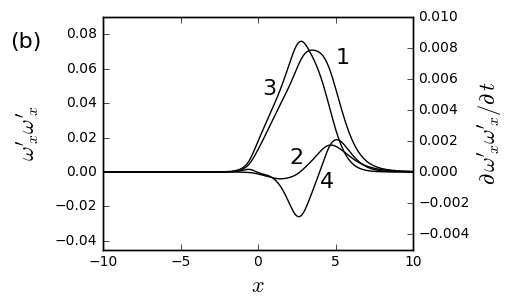
\includegraphics[width=0.5\linewidth]{xline_ox1gen.png}}
\caption{На прямой, проходящей через область, занятую продольным вихрем, при $r = 0.5, \theta = \pi/8$, приведены: (a) --- Квадрат стационарной продольной завихренности (кривая 1), вклад в его производство со стороны \eqref{time_OXgen_terms} (кривая  2) и других слагаемых в правой части уравнения \eqref{time_OX_eq} (кривая 3); (b) --- средний квадрат пульсаций продольной завихренности $\overline{\omega'_x \omega'_x}^t$ (кривая 1) и вклад в его производство со стороны \eqref{time_ox1gen_terms1} (кривая  2), \eqref{time_ox1gen_term2} (кривая  3) и других слагаемых в правой части уравнения \eqref{time_ox1_eq} (кривая  4).}
\label{xline_oxgen_pic}
\end{figure}

На рисунке \ref{xline_oxgen_pic}(a) приведено значение выделенных слагаемых на прямой, проходящей через область, занятую продольным вихрем, $r = 0.5, \theta = \pi/8$. Хотя существует небольшой участок, на котором вклад других слагаемых в правой части уравнения \eqref{time_OX_eq} (изображенный кривой 3) превосходит вклад слагаемых \eqref{time_OXgen_terms} (изображенных кривой 2), выделенные слагаемые определяют форму поля $\Omega_x^2$ (изображенного кривой 1). Таким образом, нет сомнения, что за генерацию стационарных продольных вихрей ответственна выделенная пара слагаемых. Среди слагаемых, представленных кривой 3, можно выделить конвективное слагаемое. Оно переносит $\Omega_x$ вверх по течению, о чем говорит то, что в области $x \approx 3$ оно дает отрицательный вклад, а в области $x \approx 0$ --- положительный. 

В модельном порыве, также как и в бегущей волне, оба слагаемых \eqref{time_OXgen_terms} близки друг к другу по величине. Сохраняется отмеченная в предыдущем разделе согласованность фаз между пульсациями продольной скорости $v'_x$ и продольной завихренности $\omega'_x$, однако форма пульсационной составляющей движения оказывается несколько более сложной. Согласованность фаз объясняется механизмом образования пульсаций продольной завихренности $\omega'_x$, выделенным в модельном порыве, который также совпадает с механизмом, найденным в бегущей волне. 

\begin{figure}[h!]
\center{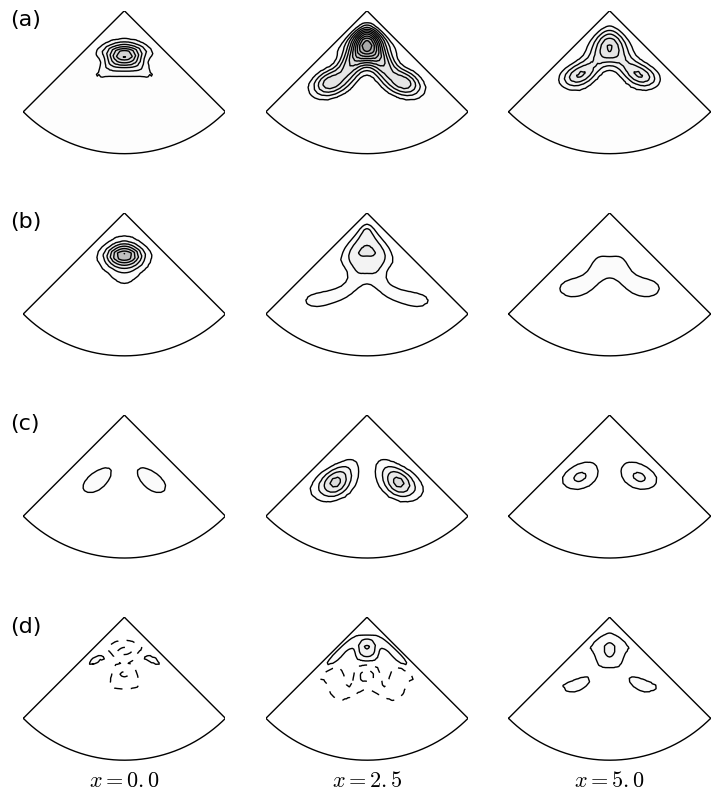
\includegraphics[width=0.9\linewidth]{puff_ox1gen.png}}
\caption{В нескольких сечения трубы изображена интенсивность пульсаций продольной завихренности $\overline{\omega'_x \omega'_x}^t$ (ряд а) и вклад в её генерацию со стороны слагаемых \eqref{time_ox1gen_terms1} (ряд b), слагаемого \eqref{time_ox1gen_term2} (ряд с) и других слагаемых в правой части \eqref{time_ox1_eq} (ряд d). Сплошные изолинии соответствуют положительным значениям, прерывистые --- отрицательным.}
\label{mp_ox1gen_pic}
\end{figure}

Выделить механизм образования пульсаций продольной завихренности $\omega'_x$ позволяет анализ уравнения, описывающего её изменение, полученного по аналогии с \eqref{ox1_eq} вычитанием \eqref{time_OX_eq} из \eqref{ox_eq}:
\begin{multline}\label{time_ox1_eq}
\pd{\omega'_x}{t} - \nu \nabla^2 \omega'_x = - (\V - \c, \nabla) \omega'_x - (\v', \nabla) \Omega_x +(\Om, \nabla) v'_x + (\om', \nabla) V_x - \\ - (\v', \nabla) \omega'_x  + (\om', \nabla) v'_x  + \overline{(\v', \nabla) \omega'_x)}^t  - \overline{(\om', \nabla)}^t
\end{multline}
Удобнее работать с уравнением, определяющим интенсивность пульсаций продольной завихренности $\overline{\omega'_x \omega'_x}^t$, полученным скалярным умножением \eqref{time_ox1_eq} на~$2 \omega'_x$ с последующим осреднением по времени. Анализ этого уравнения позволяет выделить две группы слагаемых, ответственных за образование пульсаций продольной завихренности, имеющих вид:
\begin{equation}\label{time_ox1gen_terms1}
\frac{\d \omega'_x}{\d t} = \omega'_r \frac {\d V_x}{\d r} + \frac{\Omega_\theta}{r} \frac{\d v'_x}{\d \theta} + 
\end{equation}
\begin{equation}\label{time_ox1gen_term2}
+\Omega_x \frac {\d v'_x}{\d x} + ...
\end{equation}
Слагаемые \eqref{time_ox1gen_terms1} отвечают за поворот нормальных к стенке вихрей, возникающих в пульсационной составляющей движения. Приобретая продольную составляющую эти вихри обеспечивают формирование значительных по амплитуде пульсаций $\omega'_x$ в области между полосой замедления и осью трубы. Вклад \eqref{time_ox1gen_terms1} в $\overline{\omega'_x \omega'_x}^t$ представлен на рисунке \ref{mp_ox1gen_pic} в нескольких сечения трубы. Он имеет значительную амплитуду и отвечает за формирование пульсаций $\omega'_x$ в центральной части расчетной области (распределение $\overline{\omega'_x \omega'_x}^t$ представлено на рисунке \ref{mp_ox1gen_pic} в ряду (a)). Однако на месте существования продольных вихрей влияние слагаемых \eqref{time_ox1gen_terms1} невелико. Кроме того, пульсации, формируемые слагаемыми \eqref{time_ox1gen_terms1}, согласованны по фазе с пульсациями $v'_x$ так, что их нелинейное взаимодействие, выраженное слагаемыми \eqref{time_OXgen_terms}, близко к нулю. За образование продольных вихрей ответственно слагаемое \eqref{time_ox1gen_term2}. Его вклад в $\overline{\omega'_x \omega'_x}^t$ представлен на рисунке \ref{mp_ox1gen_pic} в ряду (c). Оно создает пульсации $\omega'_x$ на месте существования продольных вихрей, согласованные с пульсациями $v'_x$ так, что их нелинейное взаимодействие эффективно поддерживает существование продольных вихрей. Другие слагаемые в правой части уравнения \eqref{time_ox1_eq} существенного влияния на интенсивность $\omega'_x$ не оказывают, их вклад в образование $\overline{\omega'_x \omega'_x}^t$ приведен в ряду (d). Можно отметить, что они включают конвективные слагаемые, обеспечивающие перенос существующих пульсаций $\omega'_x$, создаваемых слагаемым \eqref{time_ox1gen_terms1}, вниз по течению. При $x \le 0$ в области между полосой замедления и осью трубы конвективное слагаемое дает отрицательный вклад, а при $x \ge 2$ --- положительный, так как оно переносит $\omega'_x$ из первой области во вторую.

На рисунке \ref{xline_oxgen_pic}(b) приведено значение вклада в формирование $\overline{\omega'_x \omega'_x}^t$ каждой из выделенных групп слагаемых на прямой, проходящей через область, занятую продольным вихрем, $r = 0.5, \theta = \pi/8$. Как только что обсуждалось, подавляющий вклад в образование $\overline{\omega'_x \omega'_x}^t$  дает слагаемое \eqref{time_ox1gen_term2} (кривая~3). Оно определяет интенсивность пульсаций $\omega'_x$ на этой прямой (значение $\overline{\omega'_x \omega'_x}^t$ представлено кривой 1). Другие слагаемые в правой части уравнения (кривые 2, 4) существенного влияния не оказывают. Группа слагаемых, которым соответствует кривая 4, включает конвективное слагаемое, обеспечивающее перенос пульсаций $\omega'_x$ в этой области вниз по течению, в результате чего при $x \approx 3$ это слагаемое дает отрицательный вклад, а при $x \approx 5$ --- положительный. 

В этом разделе было показано, что выделенный при изучении бегущей волны механизм образования продольных вихрей, обеспечивает их формирование также и в модельном порыве. 


\section{Выводы по главе}

В предыдущей главе представлены результаты численного исследования модельного порыва, в котором было составлено представление о его внутренней структуре и механизме самоподдержания колебаний. В подвижной системе отсчета в модельном порыве выделяются стационарные полосы повышенной и пониженной скорости, вытянутые вдоль стенки трубы. Полосы образуются под действием стационарных продольных вихрей, которые формируются в результате нелинейного взаимодействия нестационарных пульсаций, возникающих из-за неустойчивости полосчатого движения. В настоящей главе представлены определяющие элементы нелинейного механизма образования продольных вихрей. Таким образом, определены все элементы цикла самоподдержания колебаний внутри модельного порыва. 

Установлено, что пульсации продольной скорости, возникающие в результате неустойчивости стационарного полосчатого движения, вызывают появление пульсаций продольной завихренности. Пульсации продольной скорости и продольной завихренности оказываются согласованными по фазе таким образом, что их нелинейное взаимодействие усиливает продольные вихри. Продольные вихри формируются на месте возникновения пульсаций, в области между полосами повышенной и пониженной скорости, оказываясь расположенными наиболее удачным образом для поддержания существования этих полос.

Пульсации возникают в результате линейной неустойчивости полосчатого течения и могут быть воспроизведены в рамках линеаризованных уравнений. Решения линейной задачи устойчивости также воспроизводят описанный выше механизм поддержания продольных вихрей, но только в том случае, когда в исследуемом на устойчивость течении учтено не только продольное, но и поперечное движение, индуцируемое этими вихрями. Невзирая на небольшую амплитуду поперечного движения, его учет необходим для адекватного описания пульсаций продольной завихренности. 

Также в главе представлена бегущая волна, возникающая на сепаратрисе в непротяженной расчетной области. Она напоминает бегущую волну, возникающую в передней части порыва, но является точной в том смысле, что её поле скорости меняется вдоль трубы и во времени строго периодическим образом. Простота поведения выделенного решения позволяет на его примере в более простой и в тоже время строгой форме продемонстрировать особенности движения, связанные с самоподдержанием колебаний.

Пример бегущей волны показывает, что механизм поддержания пульсаций в потоке может быть сформулирован и изучен в двумерной постановке в нормальной к основному потоку плоскости. Возникающие на среднем течении пульсации в линейном приближении меняются вдоль трубы по гармоническому закону и могут быть представлены двумерным полем амплитуды и фазы. Их нелинейное взаимодействие определяет форму продольных вихрей, которые также представляются двумерным полем продольной завихренности. Однородные вдоль трубы вихри приводят к образованию полос повышенной и пониженной скорости, также однородных вдоль трубы. 

Можно отметить, что выделенный механизм образования продольных вихрей схож с механизмом линейной неустойчивости. На фоне пульсаций продольной скорости в области их возникновения, где их фазовая скорость близка к скорости жидкости, поле скорости теряет устойчивость к продольным вихрям. Скорость роста стационарной составляющей продольной завихренности пропорциональная амплитуде её пульсаций, а скорость роста амплитуды пульсаций пропорциональна средней составляющей. Аналогичная неустойчивость может иметь место в следе за телом или в слое смешения. 

Полосчатые структуры являются неотъемлемой частью всех сценариев самоподдержания пристенной турбулентности. Можно ожидать, что выделенный механизм генерации продольных вихрей, поддерживающих полосчатые структуры, имеет отношение не только к турбулентным порывам в трубах, но и к более широкому классу пристенных турбулентных течений. 





